\section{Модель структуры системы}

\begin{center}
\begin{tabular}{ | m{3.5cm} | m{10cm}| }  
  \hline
  \textbf{Элемент}& \textbf{Свойство}\\
  \hline
  Оси монтировки& Выполняет функцию наведения телескопа\\
  \hline
  Основание& Выполняет несущую функцию\\
  \hline
  Труба& Выполняют функции защиты и несения оптической подсистемы\\
  \hline
  Объектив& Создаёт действительное изображение, поступающее в окуляр\\
  \hline
  Окуляр& Преобразует изображение для восприятия человеком\\
  \hline
  Фокусёр& Фокусирует изображение воздействием на окуляр\\
  \hline
\end{tabular}
\end{center}

\textbf{Взаимодействие между элементами системы}

\begin{center}
\begin{tabular}{ | m{5cm} | m{8cm}| }  
  \hline
  \textbf{Пара элементов}& \textbf{Связь между ними}\\
  \hline
  Оси монтировки и труба& Направляет\\
  \hline
  Оси монтировки& Перпендикулярны\\
  \hline
  Монтировка и труба& Установлена на\\
  \hline
  Объектив и окуляр& Передаёт изображение\\
  \hline
  Труба и оптическая подсистема& Содержит\\
  \hline
  Монтировка и основание& Установлена на\\
  \hline
  Фокусёр и окуляр& Фокусировка\\
  \hline
\end{tabular}

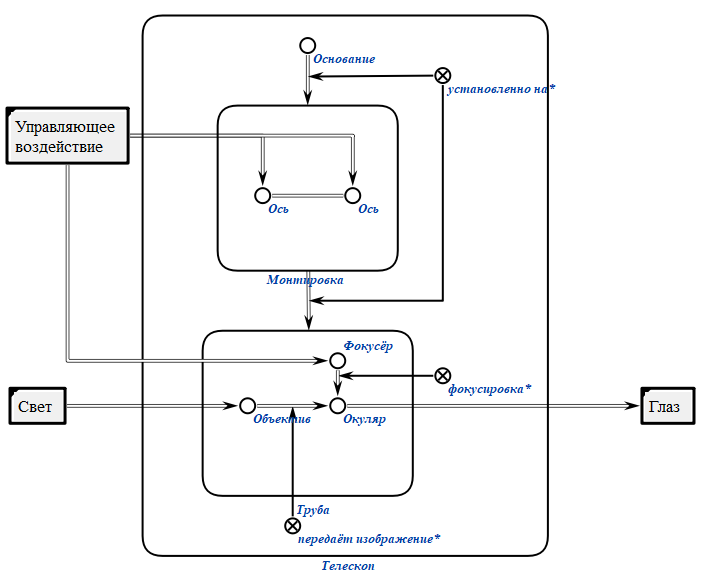
\includegraphics[]{123.png}

\end{center}
